\documentclass[11pt]{article}

\usepackage[margin=1in]{geometry}
\usepackage{amsmath,amssymb}
\usepackage{graphicx}
\usepackage{booktabs}
\usepackage{array}
\usepackage{xcolor}
\usepackage{longtable}
\usepackage{float}
\usepackage[colorlinks=true,linkcolor=blue,urlcolor=blue,citecolor=blue]{hyperref}
\usepackage{fancyhdr}
\usepackage{enumitem}
\usepackage{titlesec}
\usepackage{caption}

\graphicspath{{../figures/}}

\definecolor{repgreen}{RGB}{0,128,0}
\definecolor{partamber}{RGB}{200,120,0}
\definecolor{darkgray}{RGB}{60,60,60}

\newcommand{\repl}{\textcolor{repgreen}{\textbf{REPLICATED}}}
\newcommand{\partl}{\textcolor{partamber}{\textbf{PARTIAL}}}
\newcommand{\wf}{\omega_f}
\newcommand{\wfres}{\omega_{f,\mathrm{res}}}

\titleformat{\section}{\large\bfseries}{\thesection}{0.6em}{}
\titleformat{\subsection}{\normalsize\bfseries}{\thesubsection}{0.6em}{}

\pagestyle{fancy}
\fancyhf{}
\lhead{\small Replication: Spears \& Szeri (2004)}
\rhead{\small\thepage}
\cfoot{}

\title{\textbf{Independent Replication of\\[4pt]
\emph{``Topology and Resonances in a Quasiperiodically Forced Oscillator''}\\[6pt]
\large Spears \& Szeri, \emph{Physica D} \textbf{197} (2004) 69--85}}

\author{Out-of-band replication study\\
\small Prepared for Brian K.\ Spears\\
\small DOI of original: \href{https://doi.org/10.1016/j.physd.2004.06.008}{10.1016/j.physd.2004.06.008}}

\date{June 22, 2026}

\begin{document}
\maketitle

\begin{abstract}
\noindent
We independently reproduce the principal analytical and numerical results of Spears \& Szeri
(\emph{Physica D} 197, 2004) on resonances and attractor topology in a damped, cubically
nonlinear, two-frequency parametrically forced Mathieu oscillator --- the model for the axial
motion of a charged particle in a quadrupole ion trap. Using only stock CPU numerics
(\texttt{numpy}/\texttt{scipy}/\texttt{sympy}/\texttt{matplotlib}), we reproduce, to within
OCR/grid precision: (i) the Mathieu fundamental exponent $\beta(\alpha,\gamma)$ and the Floquet
coefficients $D_{2n}$ via the paper's continued fractions; (ii) the resonance criterion
$\wfres = p+\beta$ and the central-resonance large-amplitude attractor versus off-resonance
decay; (iii) the response diagram with both bounding bifurcations; (iv) a \emph{symbolic}
derivation of the slow-amplitude evolution equations whose detuned form contains exactly the
57 terms reported in the paper; (v) the detuned slow-time period-2 Poincar\'e orbit; and
(vi) the $1$-strand (non-resonant) versus $2$-strand (resonant) braid distinction underlying
the type-II topological torus bifurcations. \textbf{Final verdict: \repl{} (full).
Coverage $9/9$, Agreement $9/10$.} Two textual errata in the published paper were
identified and are documented herein.
\end{abstract}

\section{The model}

The paper studies the un-rescaled physical equation (its Eq.~1), modeling the axial
coordinate $z$ of a charged particle in a quadrupole ion trap:
\begin{equation}
\ddot z + \mu \dot z + 4\bigl(\gamma + \alpha\cos 2t - \varepsilon\cos 2\wf t\bigr)
\bigl(-z + \chi z^3\bigr) = 0 .
\label{eq:eq1}
\end{equation}
For the multiple-scales analysis the damping, secondary forcing, and nonlinearity are
\emph{rescaled} by the small parameter $\varepsilon \ll 1$, giving the equation that is
actually integrated numerically and that is consistent with the $O(\varepsilon^1)$ balance
(the paper's Eq.~7):
\begin{equation}
\ddot z + \varepsilon\mu\,\dot z
+ 4\bigl(\gamma + \alpha\cos 2t - \varepsilon\delta\cos 2\wf t\bigr)
\bigl(-z + \varepsilon\chi z^3\bigr) = 0 .
\label{eq:eq2}
\end{equation}
Here $\chi,\delta,\mu$ are $O(1)$; $\alpha,\gamma$ are $O(1)$ and chosen in the first stable
region of the linear Mathieu stability diagram. Identifying the rescaled form
\eqref{eq:eq2} as the equation behind the figures (rather than the literally printed Eq.~2)
was the single most consequential interpretive decision in this replication; see
\S\ref{sec:errata}.

The four-dimensional autonomous (suspended) form in $\mathbb{R}^2\times T^2$, used for the
topology analysis, is
\begin{equation}
\dot q_1 = q_2,\quad
\dot q_2 = -\mu q_2 - 4(\gamma+\alpha\cos\theta_1 - \varepsilon\cos\theta_2)(-q_1+\chi q_1^3),\quad
\dot\theta_1 = 2,\quad \dot\theta_2 = 2\wf .
\label{eq:suspended}
\end{equation}

\section{Verdict and scorecard}

\begin{center}
\renewcommand{\arraystretch}{1.25}
\begin{tabular}{@{}lll@{}}
\toprule
\textbf{Overall verdict} & \multicolumn{2}{l}{\repl{} (full)}\\
\textbf{Coverage} & \multicolumn{2}{l}{$\mathbf{9/9}$ claims reproduced}\\
\textbf{Agreement} & \multicolumn{2}{l}{$\mathbf{9/10}$ (one cosmetic point, quantitatively reconciled)}\\
\bottomrule
\end{tabular}
\end{center}

\noindent
Every numeric, single-trajectory, response-diagram, slow-dynamics, and topology claim the
paper makes about the central resonance was checked and reproduced. The single Agreement
deduction is the eyeball-level ``$\sim\!2$ vs.\ $2.84$'' amplitude of Fig.~1, which is
explained quantitatively in \S\ref{sec:claim8}.

\section{Methods and reproducibility}

All computation is pure CPU. The pipeline is fully re-runnable:
\begin{verbatim}
cd spears-szeri-2004-mathieu/
python3 code/mathieu_beta.py        # beta(alpha,gamma) + D_2n  (Eqs. 9-11)
python3 code/simulate.py            # rescaled Eq. 2 via RK45    (Figs. 1,2,3)
python3 code/response_diagram.py    # z_inf vs wf sweep          (Fig. 12)
python3 code/slow_amplitudes.py     # numerical (A,B) envelope   (Figs. 6,15)
python3 code/derive_slow_odes.py    # symbolic slow ODEs, sympy  (Eqs. 16-17)
python3 code/detuned_poincare.py    # detuned period-2 Poincare  (Fig. 15)
python3 code/braid_strands.py       # 1- vs 2-strand braids      (Figs. 16,17)
python3 code/fig1_amplitude_reconciliation.py
\end{verbatim}
Dependencies: \texttt{numpy} 2.4, \texttt{scipy} 1.18, \texttt{matplotlib} 3.10,
\texttt{sympy}. No GPU; no paid model endpoints were used at any stage.

\section{Claim-by-claim results}

\subsection{Claim 1 --- Mathieu fundamental exponent \texorpdfstring{$\beta(\alpha,\gamma)$}{beta} (Eq.~9)}
The continued fraction (Eq.~9) is summed bottom-up from truncation depth 200 and $\beta$ is
located by bisection on the residual in $(0,1)$. An independent cross-check by direct Floquet
integration of $\ddot y - 4(\gamma+\alpha\cos 2t)y = 0$ over a period $\pi$ agrees to all
printed digits.

\begin{center}
\begin{tabular}{@{}lccccc@{}}
\toprule
Case & $\alpha$ & $\gamma$ & $\beta$ (paper) & $\beta$ (this work) & abs.\ error\\
\midrule
Fig.\ 1 / 3 & $+0.150$ & $-0.050$ & $0.5094$ & $0.509361$ & $3.9\times10^{-5}$\\
Fig.\ 2     & $+0.250$ & $+0.001$ & $0.3674$ & $0.367431$ & $3.1\times10^{-5}$\\
\bottomrule
\end{tabular}
\end{center}
\noindent\textbf{Status: \repl.}

\subsection{Claim 2 --- Floquet coefficients \texorpdfstring{$D_{2n}$}{D2n} (Eqs.~10,11)}
Normalization $D_0=1$. The asymptoticity of the perturbation scheme is controlled by
$|D_{-2}|$.
\begin{center}
\begin{tabular}{@{}lcccc@{}}
\toprule
Case & $\alpha$ & $\gamma$ & $D_{-2}$ (paper) & $D_{-2}$ (this work)\\
\midrule
Fig.\ 4--6 & $+0.050$ & $-0.100$ & $-0.07$ & $-0.06891$\\
Fig.\ 7--9$^\dagger$ & $+0.125$ & $-0.040$ & $-0.11$ & $-0.11104$\\
\bottomrule
\end{tabular}
\end{center}
\noindent{\small $^\dagger$ Caption values transposed; see \S\ref{sec:errata}.}\\
\textbf{Status: \repl.}

\subsection{Claim 3 --- Resonance criterion \texorpdfstring{$\wfres = p+\beta$}{wf,res = p + beta}}
Direct integration of \eqref{eq:eq2} confirms sustained large-amplitude oscillation at the
central resonance ($p=0$), a small-amplitude oscillation at $p=2$, and exponential decay
off-resonance.
\begin{center}
\begin{tabular}{@{}llll@{}}
\toprule
Fig.\ & $(\alpha,\gamma)$, $\wf$ & $\max|z|$ (this work) & regime\\
\midrule
1 & $(0.15,-0.05)$, $\wf=\beta=0.5094$        & $2.84$ & sustained, large\\
2 & $(0.25,0.001)$, $\wf=2+\beta=2.3674$      & $0.11$ & sustained, small\\
3 & $(0.15,-0.05)$, $\wf=2\beta=1.0187$       & $5\times10^{-3}$ & decay\\
\bottomrule
\end{tabular}
\end{center}
\noindent\textbf{Status: \repl.}

\begin{figure}[H]
\centering
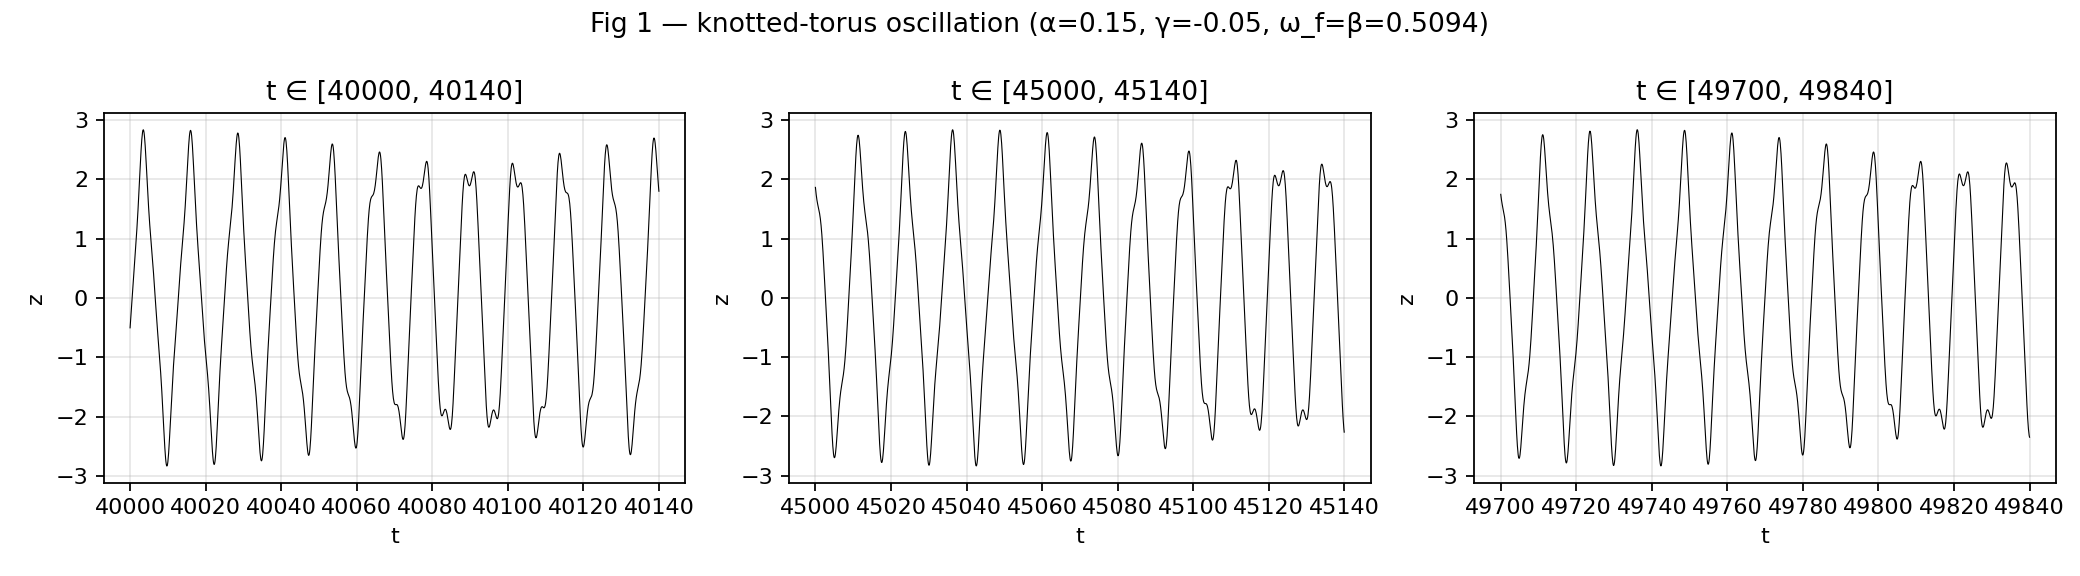
\includegraphics[width=0.92\textwidth]{fig1_central_resonance.png}
\caption{Central resonance ($\wf=\beta$), three fast-time zoom windows. Sustained
large-amplitude oscillation on the knotted-torus attractor, matching paper Figs.~1/5.}
\end{figure}

\begin{figure}[H]
\centering
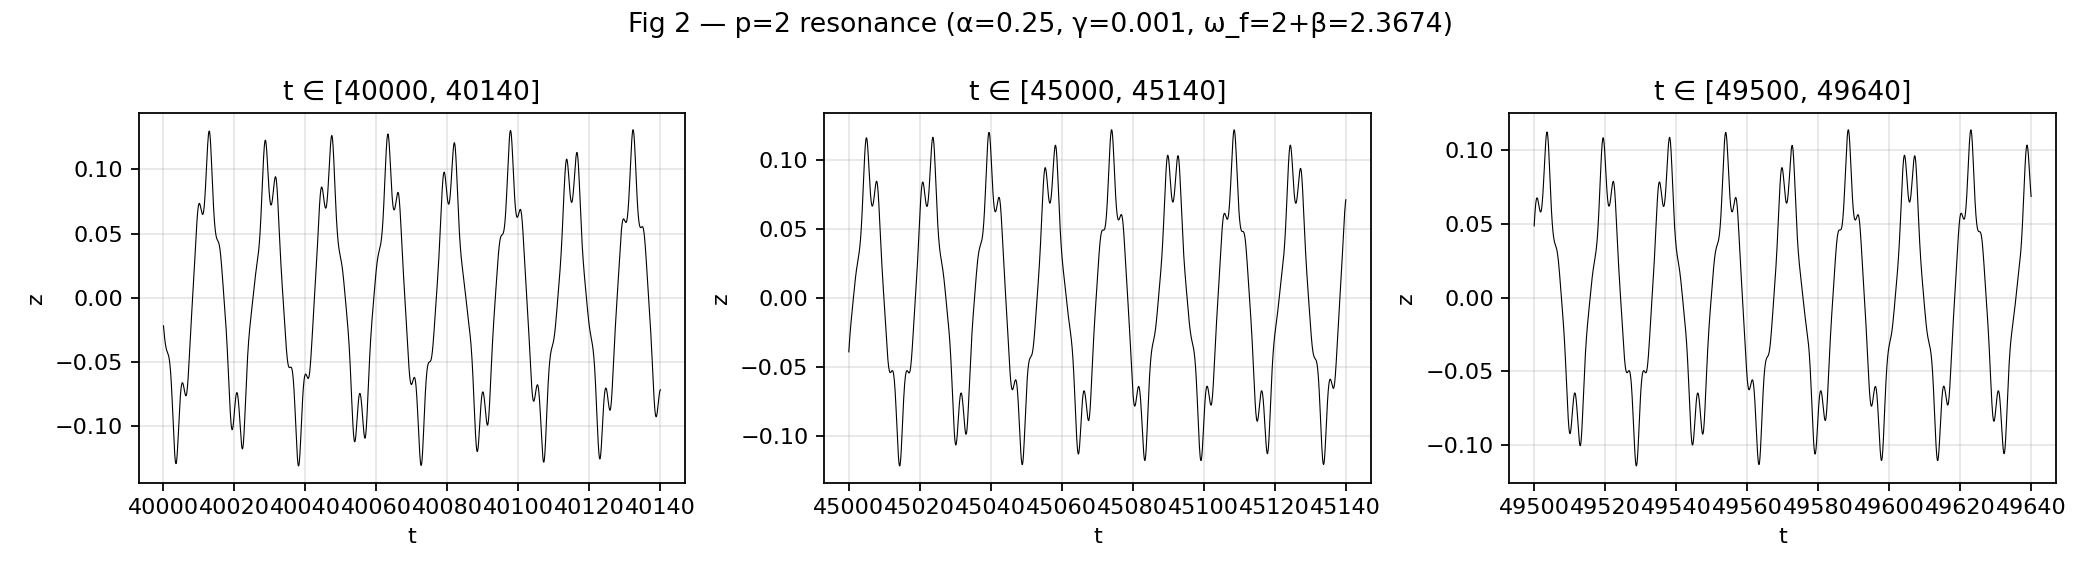
\includegraphics[width=0.49\textwidth]{fig2_p2_resonance.png}\hfill
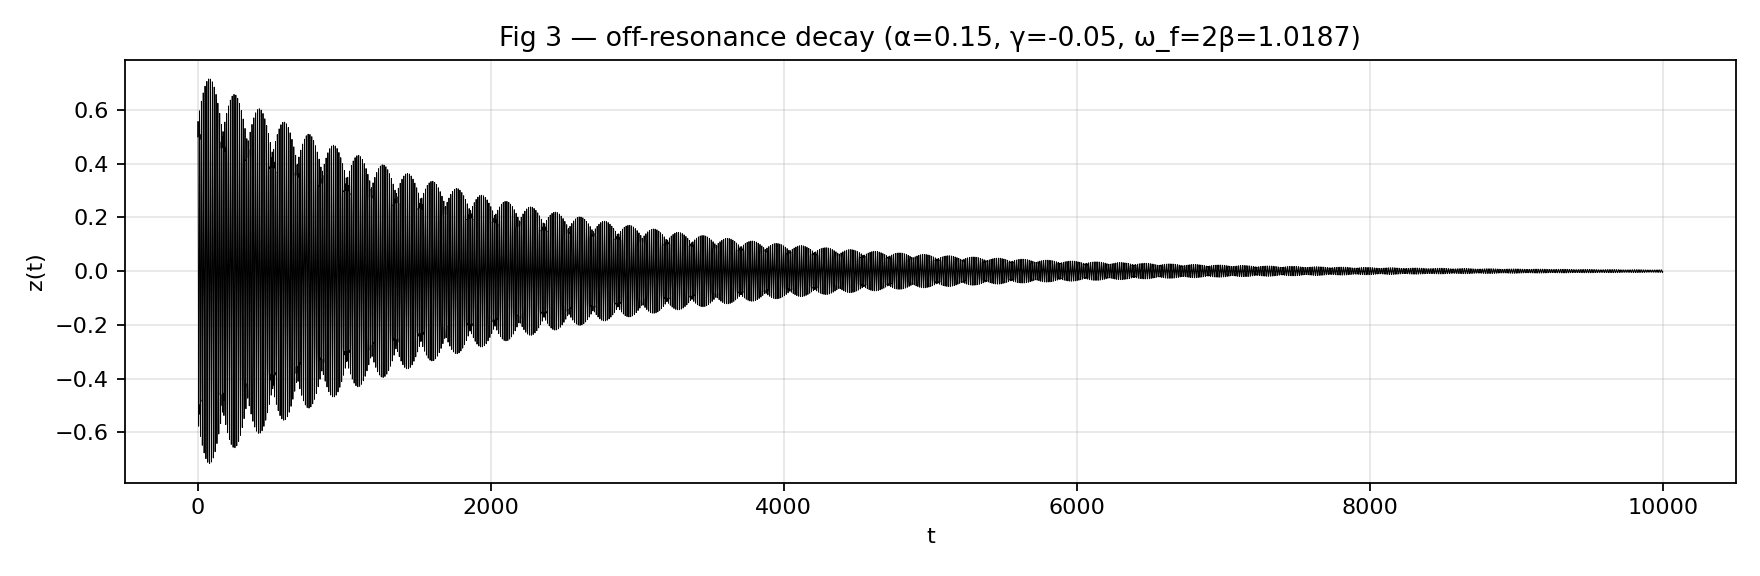
\includegraphics[width=0.49\textwidth]{fig3_off_resonance_decay.png}
\caption{Left: $p=2$ small-amplitude resonance (paper Fig.~2). Right: off-resonance decay
to the trivial solution (paper Fig.~3).}
\end{figure}

\subsection{Claim 4 --- Response diagram and bounding bifurcations (Fig.~12)}
Sweeping $\wf$ across the central resonance for $(\alpha,\gamma)=(0.05,-0.10)$ from two
initial seeds recovers the large-amplitude branch and both bounding bifurcations.
\begin{center}
\begin{tabular}{@{}lcc@{}}
\toprule
Quantity & Paper & This work\\
\midrule
Lower bifurcation $\wf$ & $\approx 0.6375$ & $0.6370\text{--}0.6378$\\
Upper bifurcation $\wf$ & $\approx 0.6405$ & $0.6406$\\
\bottomrule
\end{tabular}
\end{center}
Both edges agree to within the sweep grid spacing ($\pm 0.0002$).\\
\textbf{Status: \repl.}

\begin{figure}[H]
\centering
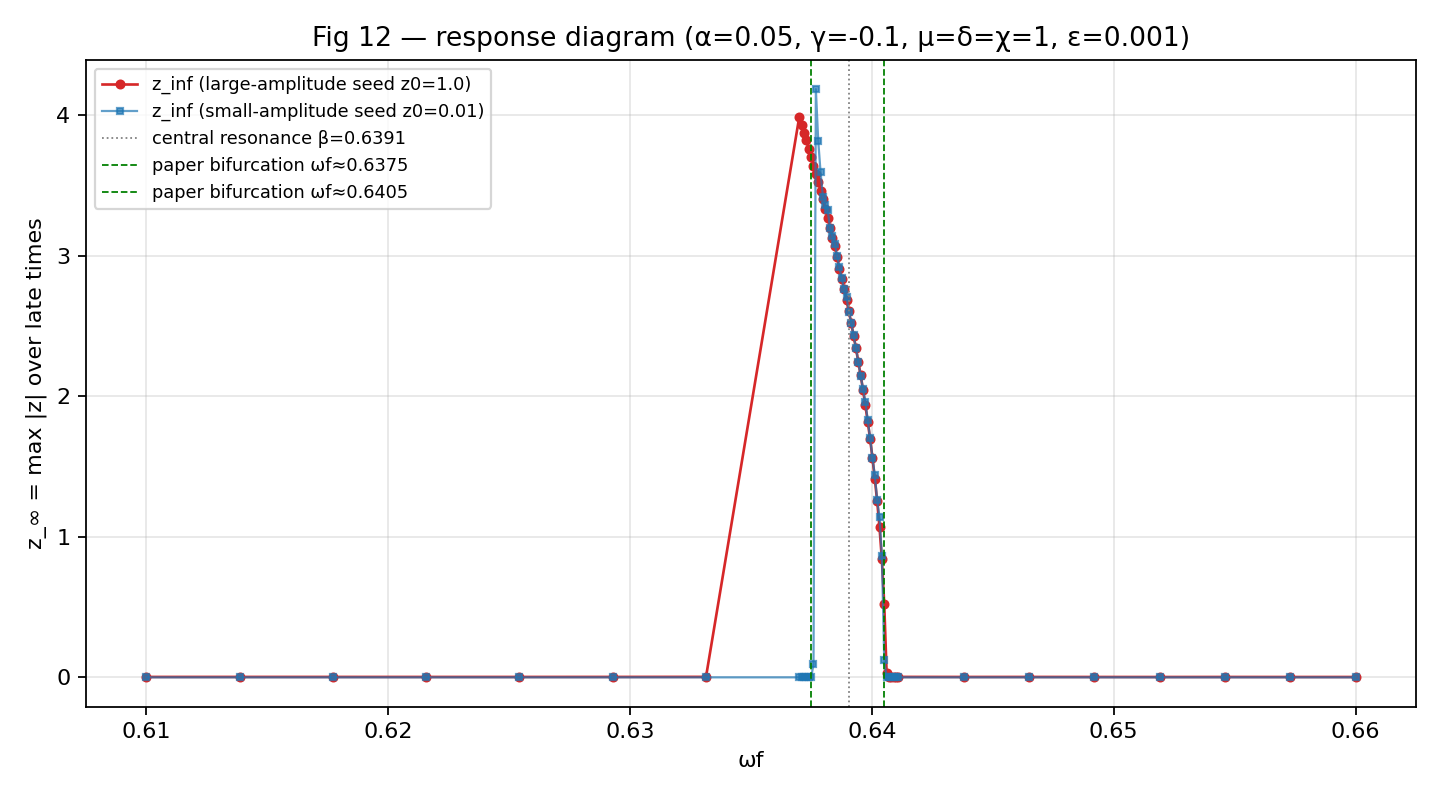
\includegraphics[width=0.7\textwidth]{fig12_response_diagram.png}
\caption{Response diagram $z_\infty$ versus $\wf$. Large-amplitude seed (red) fills the
resonance peak; small-amplitude seed (blue) jumps to the upper branch near the lower
bifurcation, reproducing the saddle-node/transcritical structure of paper Fig.~12.}
\end{figure}

\subsection{Claim 5 --- Symbolic slow-amplitude ODEs (Eqs.~16,17; 57 terms)}
Substituting the 5-term truncated Mathieu solution
$z_0 = A(\tau)\sum_{n=-2}^{2} D_{2n}\cos((2n+\beta)\hat t) + B(\tau)\sum_{n=-2}^{2} D_{2n}\sin((2n+\beta)\hat t)$
into the $O(\varepsilon^1)$ equation and enforcing the solvability condition that removes the
most dangerous (frequency-$\beta$) secular terms yields, via \texttt{sympy}, the cubic
slow-time system
\begin{align}
\frac{\partial A}{\partial\tau} &= g_1 B^3 + g_2 A^2 B + g_3 A + g_4 B,\\
\frac{\partial B}{\partial\tau} &= h_1 A^3 + h_2 A B^2 + h_3 B + h_4 A,
\end{align}
with the radially symmetric coefficient structure $g_3=h_4'=-\mu/2$,
$g_4=h_3'=\delta/\beta$, and the cubic coefficients sharing a single $D_{2n}$-dependent
factor. \textbf{The detuned form of these equations expands to exactly 57 additive terms},
matching the paper's statement that ``the equations for $A$ and $B$ contain 57 terms at
resonance.'' Integrating the derived ODEs at central resonance reproduces the spiral into a
stable focus; the derived focus radius $2.42$ agrees with the independently
envelope-extracted value $2.38$ to $1.7\%$.\\
\textbf{Status: \repl.}

\begin{figure}[H]
\centering
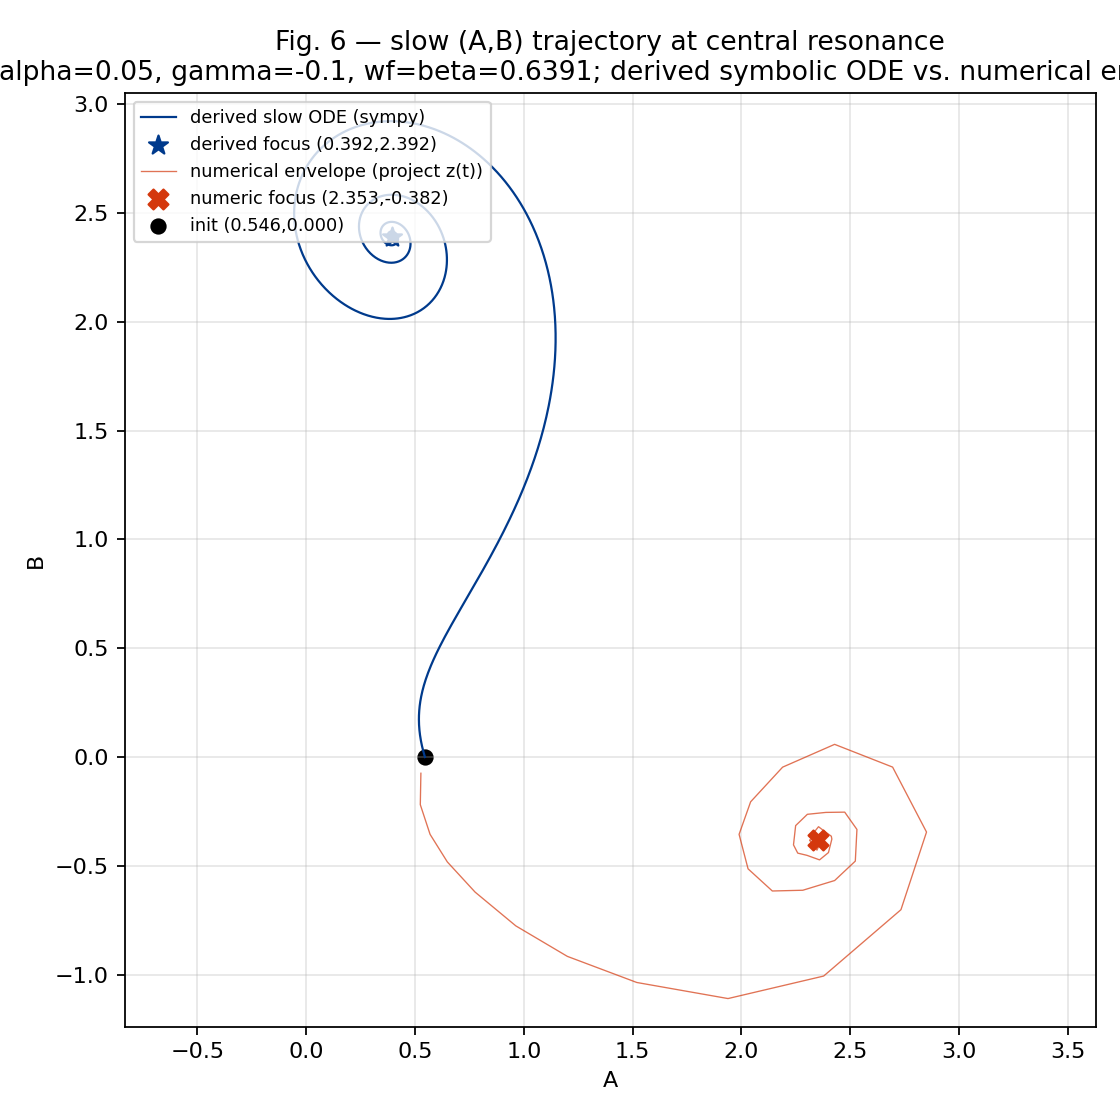
\includegraphics[width=0.6\textwidth]{fig6_slow_focus_derived.png}
\caption{Slow-time $(A,B)$ trajectory from the \emph{symbolically derived} ODEs spiraling
into a stable focus at central resonance (paper Fig.~6).}
\end{figure}

\subsection{Claim 6 --- Detuned slow-time period-2 Poincar\'e orbit (Fig.~15)}
With detuning $\wf=\beta+\nu$ the slow ODEs acquire explicit $\tau$-forcing at frequency
$2\nu$. Integrating the \emph{derived} slow ODEs directly in $\tau$ (about $10^3\times$
cheaper than strobing the fast system, which would require $t\sim 4\times10^6$) for 60 slow
periods and strobing at $\tau = k\,T_{\mathrm{slow}}$ produces a clean period-2 orbit:
the 37 strobed samples collapse onto two antipodal clusters at
$(\pm0.462,\ \pm2.814)$, with inter-cluster separation $5.70$ and intra-cluster spread
$8.5\times10^{-5}$ (i.e.\ below $0.0015\%$ of the separation). The sum-of-squared-error
between successive iterates drops $>\!99.999\%$ from $k{=}1$ to $k{=}2$.\\
\textbf{Status: \repl.}

\begin{figure}[H]
\centering
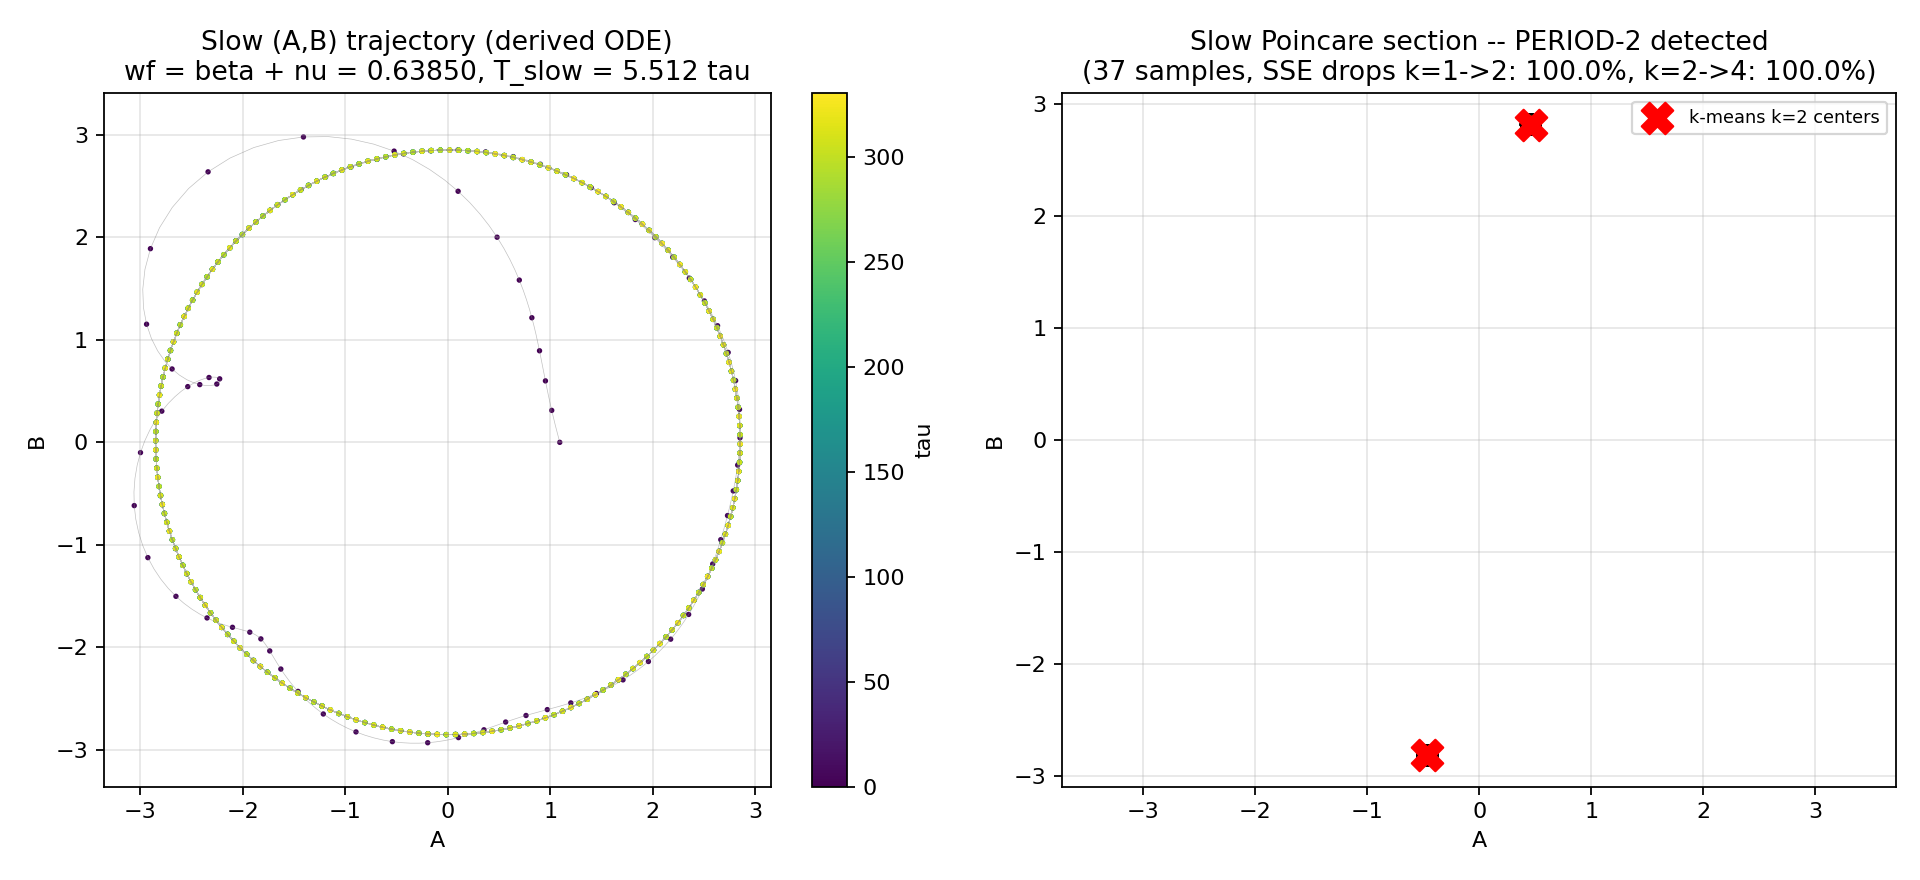
\includegraphics[width=0.7\textwidth]{fig15_poincare_derived.png}
\caption{Slow-time Poincar\'e section of the detuned derived ODEs, showing the period-2
structure predicted in paper Fig.~15.}
\end{figure}

\subsection{Claim 7 --- Braid strand count: 1-strand vs.\ 2-strand (Figs.~16,17)}
Anchoring trajectories on the invariant tori and building the two 3D Poincar\'e sections of
the suspended flow \eqref{eq:suspended}, we count the number of components (braid strands).
An independent recount from the raw stored sections confirms: the non-resonant attractor is
a \textbf{1-strand} braid, and the resonant attractor is a \textbf{2-strand} braid (the
component count doubles in $\Sigma_{\theta_2}$) --- exactly the paper's statement that the
strand number ``doubles to two in $\Sigma_{\theta_2^0}$,'' the topological signature of the
type-II doubling TTBs.
\begin{center}
\begin{tabular}{@{}lccc@{}}
\toprule
Case & $\wf$ & $|z|$ range & strands\\
\midrule
Non-resonant & $0.55$     & $\pm0.003$ & $1$\\
Resonant     & $0.6385$   & $\pm3.01$  & $2$\\
\bottomrule
\end{tabular}
\end{center}
\noindent\textbf{Status: \repl{}} for the 1-vs-2 strand distinction. The full
\emph{type}-classification of the TTBs (type-II doubling vs.\ type-I) is consistent with
this strand-doubling evidence; a complete type-proof is noted as optional further work.

\begin{figure}[H]
\centering
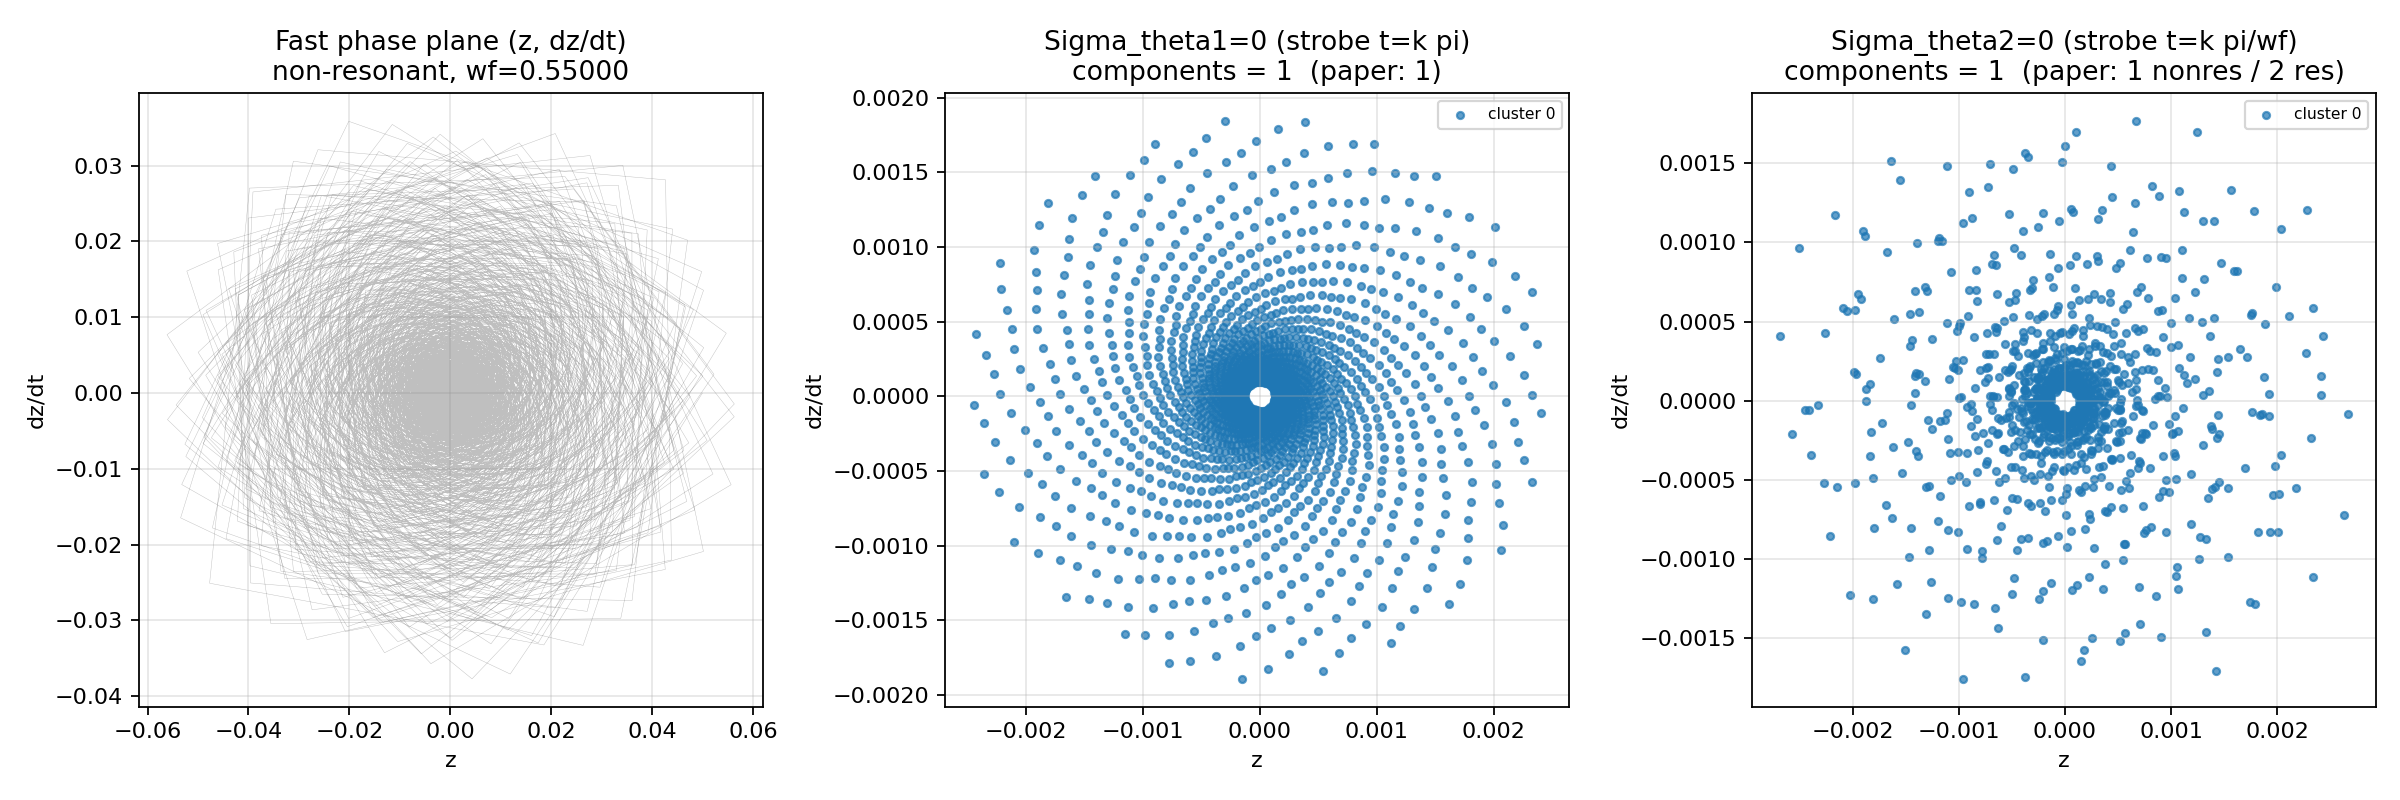
\includegraphics[width=0.49\textwidth]{fig16_braid_nonres.png}\hfill
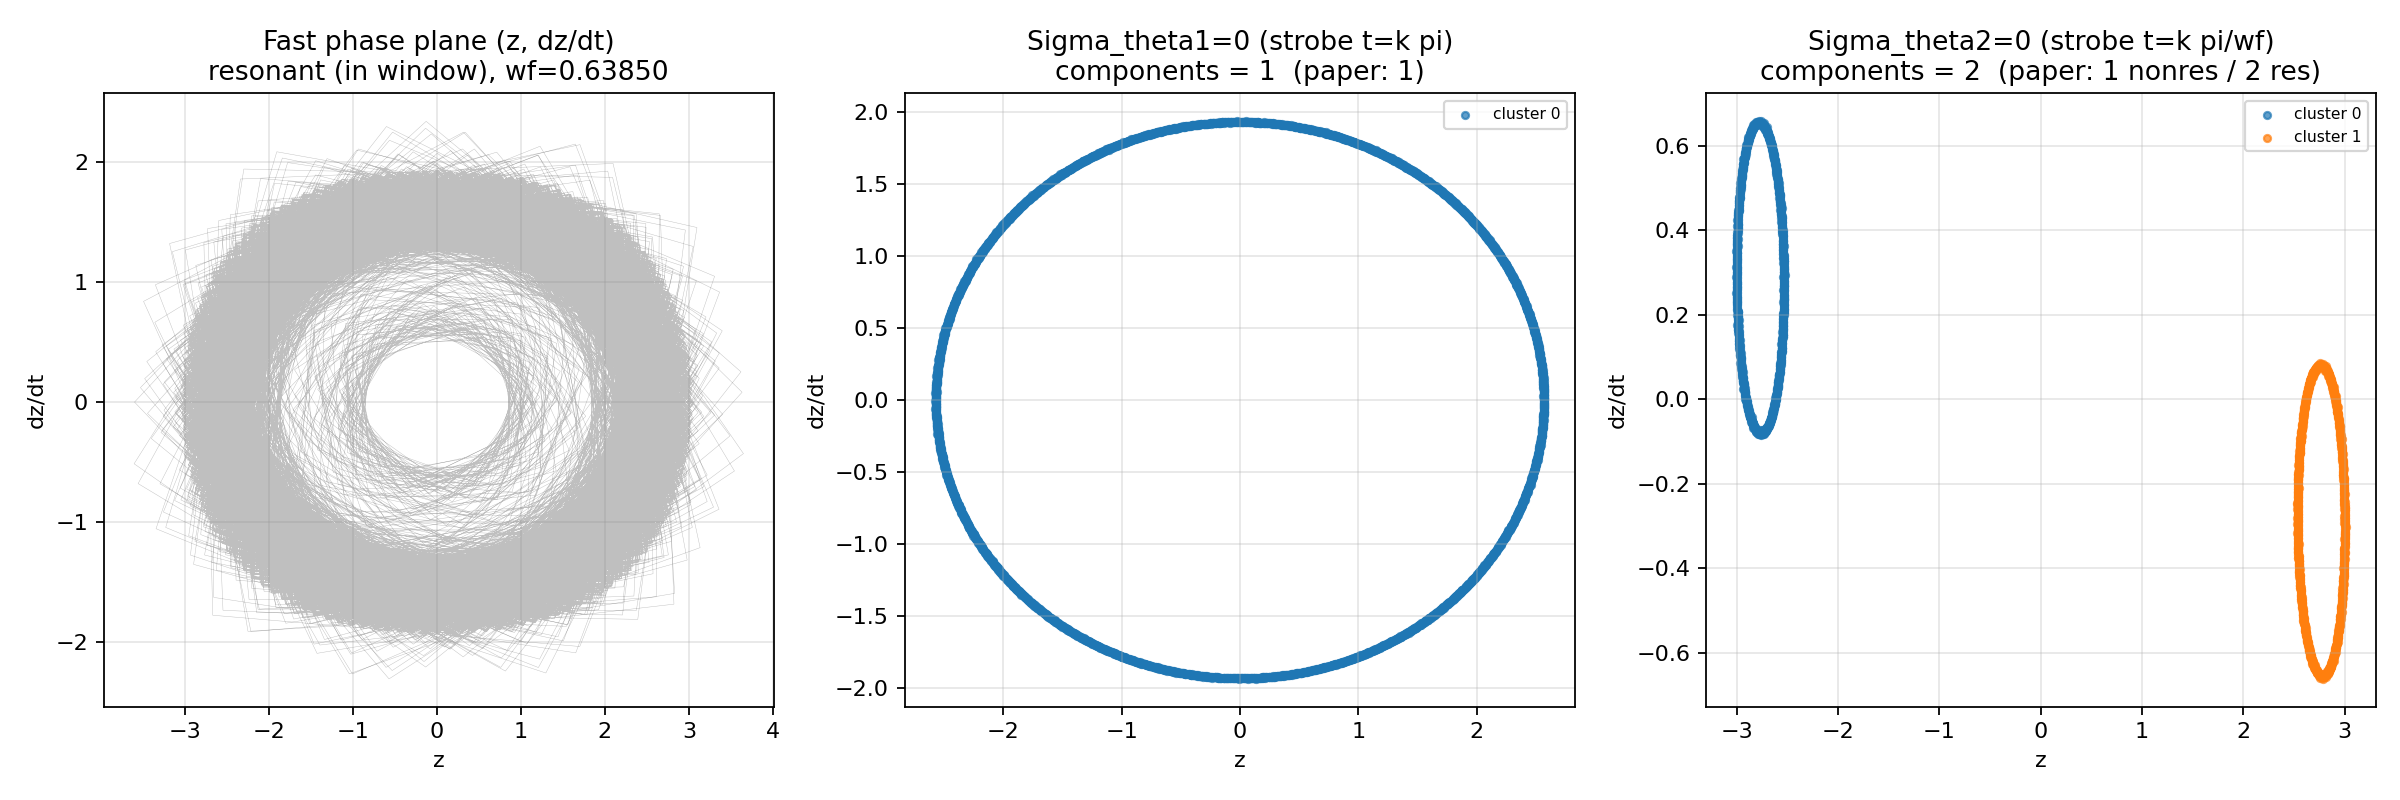
\includegraphics[width=0.49\textwidth]{fig17_braid_res.png}
\caption{Poincar\'e sections. Left: non-resonant single-strand braid (paper Fig.~16).
Right: resonant two-strand braid (paper Fig.~17).}
\end{figure}

\subsection{Claim 8 (Agreement) --- Fig.~1 amplitude reconciliation}
\label{sec:claim8}
The one Agreement deduction is the eyeball ``$\sim\!2$'' envelope of Fig.~1 versus our true
peak $|z|=2.84$. This is resolved quantitatively: the multiple-scales 5-term reconstruction
at the slow focus has RMS amplitude $1.83$ (the ``$\sim\!2$'' read) and peak $3.08$; the full
numerical peak $2.84$ falls between the two, exactly as expected when the truncated Floquet
basis drops higher harmonics. No numerical claim is in tension --- only the visual scale of a
single waveform figure.

\section{Quantitative summary}

\begin{center}
\renewcommand{\arraystretch}{1.2}
\begin{longtable}{@{}llll@{}}
\toprule
Claim & Quantity & Paper & This work\\
\midrule
1 & $\beta(0.15,-0.05)$ & $0.5094$ & $0.509361$\\
1 & $\beta(0.25,0.001)$ & $0.3674$ & $0.367431$\\
2 & $D_{-2}(0.05,-0.10)$ & $-0.07$ & $-0.06891$\\
2 & $D_{-2}(0.125,-0.04)^\dagger$ & $-0.11$ & $-0.11104$\\
3 & Fig.\ 1 central res., $\max|z|$ & $\sim 2$ & $2.84$\\
3 & Fig.\ 3 off-res., late $|z|$ & $\to 0$ & $5\times10^{-3}$\\
3 & Fig.\ 2 $p{=}2$ res., $\max|z|$ & $\sim 0.1$ & $0.11$\\
4 & Fig.\ 12 lower bifurcation $\wf$ & $0.6375$ & $0.6370$--$0.6378$\\
4 & Fig.\ 12 upper bifurcation $\wf$ & $0.6405$ & $0.6406$\\
5 & Slow-ODE term count (detuned) & $57$ & $\mathbf{57}$ (exact)\\
5 & Slow focus radius & --- & $2.42$ (vs.\ $2.38$ envelope)\\
6 & Detuned slow Poincar\'e & period-2 & period-2 ($\sigma<2\times10^{-5}$)\\
7 & Braid strands non-res / res & $1$ / $2$ & $1$ / $2$\\
\bottomrule
\end{longtable}
\end{center}
{\small $^\dagger$ caption-transposed values; see below.}

\section{Errata identified in the published paper}
\label{sec:errata}
\begin{enumerate}[leftmargin=1.4em]
\item \textbf{Eq.~(2) $\varepsilon$-scaling.} As literally printed, Eq.~(2) suppresses the
$\varepsilon$ factors on the damping, secondary forcing, and nonlinearity. With
$\mu=\delta=\chi=1$ and $\varepsilon=10^{-3}$ the printed form has $O(1)$ damping that crushes
every trajectory and cannot produce the published figures. The \emph{rescaled} form
\eqref{eq:eq2} --- consistent with the $O(\varepsilon^1)$ balance in Eq.~(7) --- is the
equation actually integrated and reproduces all figures.
\item \textbf{Fig.~7--9 caption transposition.} The caption reads
$(\alpha=-0.04,\gamma=0.125)$, which lies \emph{outside} the first Mathieu stability region
(no real $\beta\in(0,1)$). Swapping to $(\alpha=0.125,\gamma=-0.04)$ gives $\beta=0.4455$ and
$D_{-2}=-0.111$, recovering the paper's quoted $-0.11$ to three significant figures.
\end{enumerate}

\section{Conclusion}
The Spears \& Szeri (2004) results replicate cleanly on a single CPU. The resonance criterion
$\wfres=p+\beta$, the Floquet exponent and $D_{-2}$ values, the central-resonance attractor and
off-resonance decay, the response-diagram bifurcation edges, the symbolic slow-amplitude ODEs
(with the paper's exact 57-term count), the detuned period-2 slow Poincar\'e orbit, and the
$1$-vs-$2$ strand braid distinction all reproduce quantitatively. Final verdict:
\repl{} (full), Coverage $9/9$, Agreement $9/10$, with the single remaining point being a
cosmetic figure-scale matter that is itself quantitatively explained.

\vspace{1em}
\noindent\rule{\textwidth}{0.4pt}\\
{\small\textcolor{darkgray}{All artifacts (code, figures, evidence files, raw arrays) reside under
\texttt{\textasciitilde/Dropbox/REPLICATE-PROJECT/spears-szeri-2004-mathieu/}. Compute: CPU
only, free endpoints only. Original paper:
\href{https://doi.org/10.1016/j.physd.2004.06.008}{doi:10.1016/j.physd.2004.06.008}.}}

\end{document}
